\documentclass[10pt,twocolumn]{article}
\usepackage[letterpaper,margin=0.75in]{geometry}
\usepackage[T1]{fontenc}
\usepackage[utf8]{inputenc}
\usepackage{mathptmx,amsmath,amssymb,booktabs,graphicx,microtype,xcolor}
\usepackage{caption,placeins}
\usepackage[numbers,sort&compress]{natbib}
\usepackage{xurl}
\usepackage[hidelinks]{hyperref}
\urlstyle{same}
\hypersetup{pdftitle={TRACE: Area-Aware Contextual Allocation and Its Limits},
  pdfauthor={Research draft},pdfsubject={Controlled evaluation of OVSS test-time adaptation}}
\captionsetup{font=small,labelfont=bf,skip=5pt}
\setlength{\columnsep}{0.25in}
\setlength{\parindent}{1em}
\setlength{\parskip}{0pt}
\setlength{\emergencystretch}{1em}
\renewcommand{\topfraction}{0.95}
\renewcommand{\bottomfraction}{0.9}
\renewcommand{\textfraction}{0.03}
\renewcommand{\floatpagefraction}{0.75}
\setcounter{topnumber}{4}
\setcounter{totalnumber}{6}
\makeatletter
\setlength{\@fptop}{0pt}
\makeatother
\newcommand{\method}{TRACE area\_C}
\newcommand{\miou}{\mathrm{mIoU}}
\newcommand{\ObjFull}{32.441}
\newcommand{\ObjNoRegion}{32.369}
\newcommand{\ObjDelta}{+0.073}
\newcommand{\ObjLow}{-0.092}
\newcommand{\ObjHigh}{+0.244}
\newcommand{\PCFull}{28.836}
\newcommand{\PCNoRegion}{28.892}
\newcommand{\PCDelta}{-0.057}
\newcommand{\PCLow}{-0.123}
\newcommand{\PCHigh}{+0.010}


\title{TRACE: Area-Aware Contextual Allocation\\
and Its Limits in Open-Vocabulary Segmentation}
\author{Research Draft}
\date{17 November 2026}
\begin{document}
\maketitle

\begin{abstract}
Context-dependent confidence motivates alternative allocation of test-time
updates, but contextual self-support need not predict beneficial adaptation.
We study \method, a training-calibrated episodic system retaining global pixel
and CLS entropy while adding an area-aware regional bonus from fixed,
region-preserving background views. Against fixed official MLMP, the selected
system improves all eight declared L14 clean means and all fifteen severity-5
corruption means, with a 2.109-point corruption macro gain, but regresses on
B16 Object and PC60. We complete 126 training-diagnostic control cells, two
full-population component controls, 126 foreground-preserving background
interventions, six official TENT tasks, and a time-only budget study.
The full regional-term effects are \ObjDelta{} points on Object and
\PCDelta{} on PC60; both paired 95\% intervals include zero. Both full
time-budget accuracy contrasts also include zero. These findings separate a
useful selected operating point from an unestablished C-specific mechanism.
We retain negative transfer, beneficial context, historical risk-prediction
nulls, unequal calibration budgets, PC development exposure, an unresolved
Object paper-value discrepancy, and uncertainty that cannot be identified
from the original crossed update episodes. The evidence does not establish
calibrated update reliability, universal transfer, or equal-budget superiority.
\end{abstract}

\section{Introduction}
Open-vocabulary semantic segmentation transfers language--image representations
to dense prediction without restricting inference to a fixed learned class
head. CLIP provides a general representation \citep{radford2021clip}, while
segmentation-specific readouts such as NACLIP improve spatial localization
\citep{hajimiri2025naclip}. Test-time adaptation can additionally change a
model using unlabeled test inputs. Its attraction is practical, but its
self-supervised objective is only a proxy for segmentation quality.

Contextual confidence is a plausible source of proxy failure. A predicted
region can remain confident because its surroundings reinforce a class, and
minimizing that prediction's entropy can reinforce an error. The converse
also matters: context often contains useful evidence. A method should not
assume that every background dependence is harmful, or equate a context-view
score with the probability that an update improves segmentation.

We examine an area-aware allocation rule on top of the MLMP adaptation system
\citep{noori2025mlmp}. Predicted connected regions are selected at the initial
model. Each region is preserved while its complement is altered, and the
initial model's retained query support supplies a fixed regional score C.
The current method retains global pixel and CLS entropy; its regional bonus
is normalized over the whole image grid. It is not the older region-only,
image-normalized objective, and C does not decide whether an image receives
its selected update budget.

The central experimental question is attribution, not just the final score.
The selected system changes several operating fields relative to untuned
paper MLMP. We therefore separate the full-system benchmark, the matched
default-parameter C addition, selected-parameter remove/replace controls,
full-population regional-term ablations, and independently selected time
budgets. The resulting evidence supports a bounded empirical system finding:
the selected operating point can outperform fixed MLMP, but neither the
regional component nor equal-budget accuracy superiority is established by
the two full component and time studies. These negative and null results
are part of the contribution of this evaluation, not omitted exceptions.

\begin{figure*}[t]
  \centering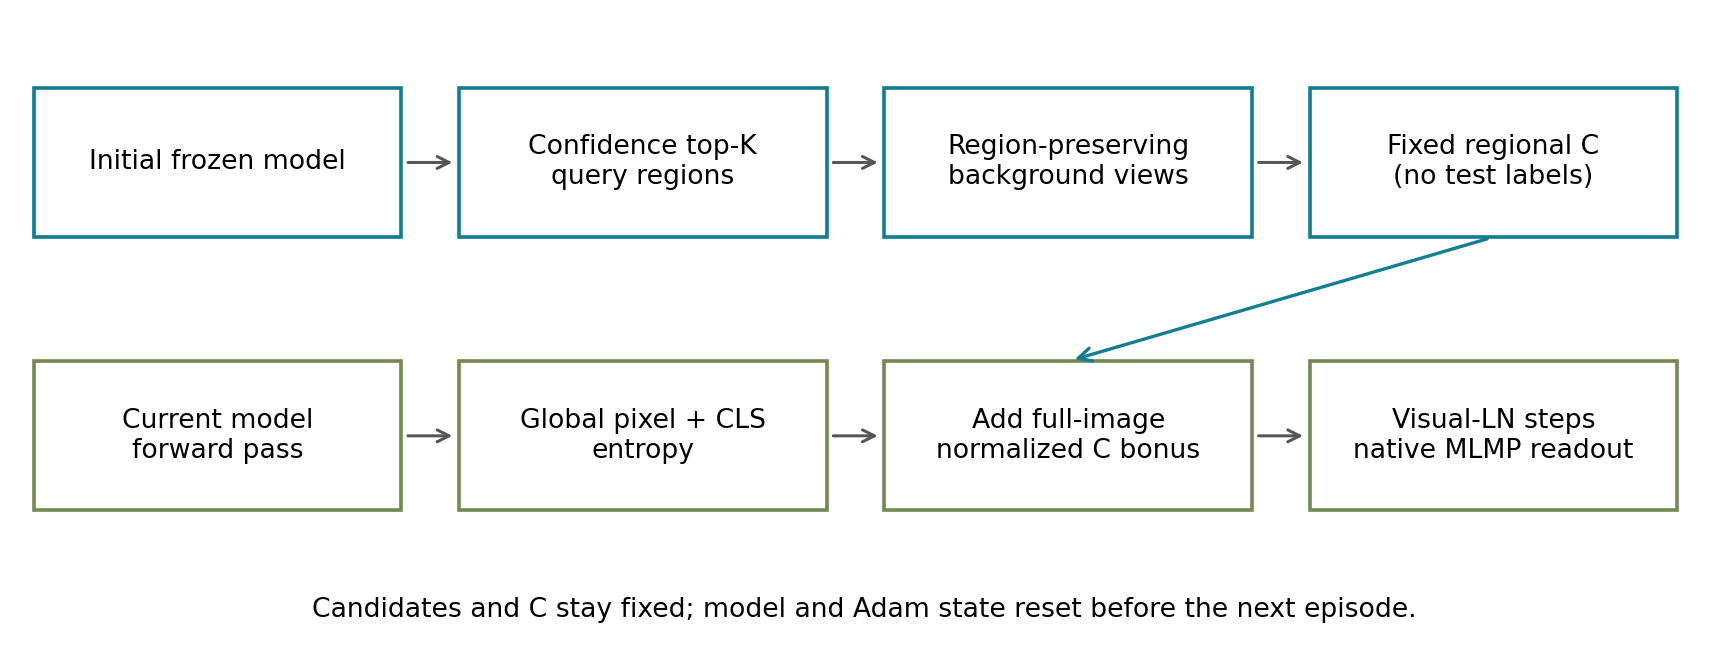
\includegraphics[width=\textwidth]{figures/pipeline.png}
  \caption{Current \method{} pipeline. Initial-model candidates and C stay fixed
  within each episode. The update retains global pixel and CLS entropy and adds
  a full-image-normalized regional bonus. Model and optimizer state reset before
  the next episode. The final native MLMP readout is unchanged.}
  \label{fig:pipeline}
\end{figure*}

\section{Related Work}
Entropy minimization is an established adaptation mechanism, not a new
objective introduced here. TENT adapts normalization parameters from test
entropy \citep{wang2021tent}. MLMP specializes adaptation to open-vocabulary
segmentation by combining intermediate visual features, multiple prompt
templates, and pixel/CLS entropy \citep{noori2025mlmp}. Our fixed baseline is
the original MLMP implementation, not an independently improvised surrogate.
The six TENT cells use the original TENT class supplied in that same
segmentation codebase.

View-based confidence requires a precise intervention definition. DeYO uses
object-destructive views and pseudo-label probability difference for sample
selection and weighting \citep{lee2024deyo}. Our fixed Region-PLPD control is
a regional adaptation, not a complete DeYO reproduction. The main C rule
instead preserves a predicted region and alters its complement. Neither
operation by itself makes a causal identification claim about beneficial
updates. A GT-free quantile map to C is also not correctness calibration
\citep{guo2017calibration}.

Context and group shifts motivate additional evaluation but do not define
interchangeable metrics. Pascal Context studies contextual dense labels
\citep{mottaghi2014context}; COCO and COCO-Stuff distinguish objects and stuff
\citep{lin2014coco,caesar2018cocostuff}. Group-shift work motivates reporting
rare groups rather than average performance alone \citep{sagawa2020dro}.
Our local Waterbirds-Seg extension measures segmentation, not standard
Waterbirds classification accuracy. The fifteen corruption operators follow
the common-corruption evaluation tradition \citep{hendrycks2019corruptions},
but are applied to VOC images in the declared MLMP-derived protocol.

\section{Current Method}
\subsection{Initial Candidates and Contextual Support}
For an episode of images $x_1,\ldots,x_B$, let $\theta_0$ be the initial
model and $q$ a raw text query. We take the query argmax on the initial dense
grid, form connected components, and retain up to $K$ regions per image in
descending mean confidence, with frozen area and confidence thresholds.
These candidates are fixed during the episode. They are not GT objects,
and confidence preselection can exclude regions that C never evaluates.

Let $m_{ir}$ denote a selected region mask. In RGB coordinates, a view keeps
the mask pixels unchanged and transforms its complement by a fixed
contrast/channel operation. If $\mu_i$ is the per-channel image mean and
$D_{\rho,\pi}(x_i)=\operatorname{clip}_{[0,255]}
\bigl(\pi[\mu_i+\rho(x_i-\mu_i)]\bigr)$ is the contrast transform with channel
permutation, the view is
\begin{equation}
 \widetilde x_{ir}=m_{ir}\odot x_i+
             (1-m_{ir})\odot D_{\rho,\pi}(x_i).
\end{equation}
Masks expand from the actual feature grid by nearest-neighbor interpolation.
The C score is the initial model's mean probability for the region's original
query $q_{ir}$ on its preserved support:
\begin{equation}
 C_{ir}=\frac{1}{|R_{ir}|}\sum_{u\in R_{ir}}
       p_{\theta_0}(q_{ir},u\mid\widetilde x_{ir}).
\end{equation}
Candidate and C temperatures are explicit selected fields. C is a heuristic
context-conditioned self-support score, not an estimated probability of
correctness or positive update utility.

\subsection{Area-Aware Regional Bonus}
Let $P$ be the adaptation prompt-prefix count, $A$ the dense-grid area,
and $H$ the entropy over raw query probabilities. With disjoint selected
components, define $w_i(u)=\sum_r\mathbf{1}[u\in R_{ir}]C_{ir}^{\gamma}$.
The current objective is
\begin{align}
 \mathcal L &=\mathcal L_{\rm pix}+
     \alpha\mathcal L_{\rm cls}+\lambda\mathcal L_{\rm reg},\label{eq:objective}\\
 \mathcal L_{\rm pix}&=\frac{1}{BPA}\sum_{i,t,u}H(p^t_\theta(u\mid x_i)),\\
 \mathcal L_{\rm cls}&=\frac{1}{BP}\sum_{i,t}H(p^t_{\theta,\rm cls}(x_i)),\\
 \mathcal L_{\rm reg}&=\frac{1}{BPA}\sum_{i,t,u}w_i(u)H(p^t_\theta(u\mid x_i)).
\end{align}
Pixel and CLS temperatures are applied before entropy. The regional sum
divides by the full grid, not by the number of region pixels or by $\sum_r C_r$.
Thus larger regions carry proportionate pixel mass, and smaller absolute C
reduces the regional bonus. Global pixel and CLS terms still update the
image for the selected number of steps. This is not an absolute update gate.

\subsection{Optimization and Native Readout}
We optimize the native visual LayerNorm parameter set with Adam and restore
both model and optimizer state between episodes. Other parameters and text
features stay fixed. The adaptation layer fraction selects feature outputs;
it does not mean that only that fraction of parameters is trainable. The same
numeric fraction maps to each backbone's actual depth.

The final readout remains native MLMP: seven-prompt-average text embeddings,
adaptive weighted aggregation of the prescribed visual layers, original
patch reconstruction, and max-over-alias semantic decoding. Adaptation
prompt-prefix changes do not silently change this final readout. Candidate
regions are formed on raw queries; the semantic-candidate control changes
that construction explicitly. For example, Object has 113 queries for 81
classes, whereas PC60 has an identity 60-query/60-class mapping.

\subsection{Training Calibration Is a Separate Budget}
The adopted system has one selected 22-field configuration per L14 clean
dataset. The operational screen covers learning rate, steps, batch size
including 8/16, loss weights, candidates, views, temperatures, feature/prompt
selection, and Adam fields through bounded one-factor and joint designs.
This is not exhaustive Cartesian optimization. Refinement and confirmation
use declared training panels; all matching B16 and VOC20 corruption fields
are then copied unchanged. All exact selected values are in the supplement
and machine-readable results.

This calibration uses a different development-information and search budget
from untuned MLMP. Although online adaptation sees no labels, the overall
method-development procedure is not training-data-free. Earlier B16 and
corruption searches were inspected before the final clean-only transfer
policy and are disclosed rather than relabeled as never exposed.

\section{Evaluation Protocol}
\subsection{Populations and Baselines}
The main comparison contains six canonical L14 segmentation conditions,
two declared local extensions, three matching B16 conditions, and all fifteen
VOC20 severity-5 corruptions: 26 conditions, three arms, and three shuffled
orders. Pascal VOC uses the declared 20/21-class variants
\citep{everingham2015pascal}; corrected Pascal Context uses the author-reference
5104-image population. Object and Stuff have 5000 images each, VOC has 1449,
local COCO-CD has 500, and local Waterbirds-Seg has 2568 declared test images.

Official MLMP remains learning rate 0.001, ten steps, batch two, CLS coefficient
one and seven prompts throughout. It is not tuned to match a target score.
Official NoAdapt and TENT use their original single reference prompt and
last-layer readout. Their contrast with MLMP is a system comparison, not a
pure adaptation-update effect. Six full clean TENT cells complete the
authorized canonical-baseline scope; no missing TENT cell is treated as zero.

\subsection{Controls and Label Isolation}
Seven diagnostic tasks use 256 training sources per family, disjoint from
the actual official evaluation IDs and physical aliases, plus separate
64-source GT-free calibration panels for score maps. Fourteen core controls
cover global/CLS/region removals, mass-matched constant/shuffled weighting,
semantic candidates and top-$K$. Seven additional fixed score-source controls
run on Object/PC60 for both backbones, giving all 126 task/control cells.
No new control is selected as the main method.

Full Object/PC60 component studies remove only the regional term under the
selected configuration. They were frozen after training diagnostics and
historical main means had been seen, before their full no-region outcomes.
The exposed chronology is explicit. Predictions are label-isolated, sealed
and successfully exited before a separate CPU GT stage. Actual finite
first-four-image loss/parameter/logit checks use tolerance $10^{-5}$ and
zero changed decoded labels before model execution proceeds.

\subsection{Dependence-Aware Uncertainty}
Multiple images can share an optimizer update, and repeated shuffled
arrangements create dependence across many images. The original TRACE/MLMP
three-order comparisons connect each population into one component. We do
not invent image-iid intervals or subtract independent marginal intervals
for those main contrasts. Three-order standard deviations are not CIs.

New controls keep episodes inside common eight-source blocks; the R04
intervention uses four-source blocks. Ten thousand shared whole-block draws
pair both arms and all orders, recomputing pooled class IoU and valid-class
omission inside each draw. Common blocks conservatively contain all actual
shared-update components; singleton-batch repetitions are not new independent
sources. Intervals are pointwise and unadjusted, conditional on fixed runs,
not independent-initialization uncertainty. Undefined draws are retained.

\subsection{Exposure and Reproduction Boundaries}
Correcting Pascal Context exposed overlap with earlier calibration:
PC59 screen/refine/confirm contain 33/62/59 reference-validation IDs and PC60
34/61/61. Fixed parameters were retained, but these are not untouched TRACE
PC tests. Waterbirds-Seg is a locally rendered extension with 2458 training,
296 validation and 2568 test images; the test is balanced at 642 per group.
Earlier 5322-image mixed-split outcomes were exposed. COCO-CD is also a local
declared extension, not a new independent official benchmark reproduction.

Original source, transforms, vocabulary, ignore and metric paths are pinned,
but the Object paper-value discrepancy remains unresolved: L14 NoAdapt is
25.03 versus 23.80 in the reference, and MLMP is 30.42 versus 28.84. Corrected
PC60 NoAdapt matches 24.95. Strict deterministic execution and workers-zero
I/O are declared extensions; historical reused baseline stages keep their
original runtime provenance. Source fidelity and scalar agreement are not
treated as sufficient proof of complete protocol equivalence.

\section{Results}
\subsection{Selected-System Performance}
Tables~\ref{tab:clean} and~\ref{tab:corruptions} contain all main conditions.
The selected area\_C system exceeds fixed MLMP on all eight declared L14
clean means and every corruption mean. The corruption arithmetic macro is
79.6800 versus 77.5711, a 2.1089-point gain. This is not an equal-search-budget
or universal SOTA claim. B16 Object regresses by 0.7367 points and PC60 by
0.4133; B16 VOC20 improves by 0.2567. Negative transfer remains part of the
result. All six original TENT means are below both selected area\_C and MLMP
on the corresponding canonical clean populations.

\begin{table*}[t]
\centering\small
\caption{Full declared clean populations. Means average official per-trial rounded mIoU. Delta is TRACE minus MLMP in percentage points. Missing TENT cells were not run in the six-cell scope.}
\label{tab:clean}
\setlength{\tabcolsep}{4pt}
\begin{tabular}{lrrrrrr}
\toprule
Condition & N & NoAdapt & TENT & MLMP & TRACE & Delta \\
\midrule
L14 Object & 5000 & 25.0300 & 26.0533 & 30.4200 & 32.4400 & +2.0200 \\
L14 PC60 & 5104 & 24.9500 & 25.2800 & 27.9833 & 28.7133 & +0.7300 \\
L14 VOC20 & 1449 & 75.9100 & 76.9967 & 83.8033 & 86.1200 & +2.3167 \\
L14 VOC21 & 1449 & 45.1300 & 45.6433 & 50.7600 & 51.1433 & +0.3833 \\
L14 PC59 & 5104 & 28.2300 & 28.7233 & 31.9433 & 32.8767 & +0.9333 \\
L14 Stuff & 5000 & 18.3400 & 18.7567 & 21.2500 & 21.9933 & +0.7433 \\
L14 Waterbirds-Seg & 2568 & 45.3700 & -- & 49.9033 & 54.0267 & +4.1233 \\
L14 COCO-CD & 500 & 62.0600 & -- & 72.3967 & 77.3833 & +4.9867 \\
\midrule
B16 Object & 5000 & 29.5900 & -- & 30.5267 & 29.7900 & -0.7367 \\
B16 PC60 & 5104 & 28.9000 & -- & 29.6133 & 29.2000 & -0.4133 \\
B16 VOC20 & 1449 & 77.5900 & -- & 84.1233 & 84.3800 & +0.2567 \\
\bottomrule
\end{tabular}
\end{table*}


\subsection{Does C Explain the Gain?}
The full-population regional-term controls do not establish a C-specific
mIoU benefit (Table~\ref{tab:full-component}). Object is \ObjFull{} with C
and \ObjNoRegion{} without it: \ObjDelta{} points, 95\% CI
$[\ObjLow,\ObjHigh]$. PC60 is \PCFull{} with C and \PCNoRegion{} without:
\PCDelta{} points, CI $[\PCLow,\PCHigh]$. Both intervals include zero.
Object's entire selected-C sourcewise integer-count arrays equal the original
main C result. PC60's new common-block episodes differ from its original
global shuffles, so its new mean does not replace the main table.

The no-region operating point retains much of the point improvement over
fixed paper MLMP. It also retains selected learning rate, batch, steps, CLS
and temperature fields. Consequently the full-system advantage cannot be
attributed to C from this comparison, nor decomposed into causal percentages
for individual hyperparameters. A null interval is not proof of exact
equivalence or absence of benefit at every possible setting.

\begin{figure*}[p]
 \centering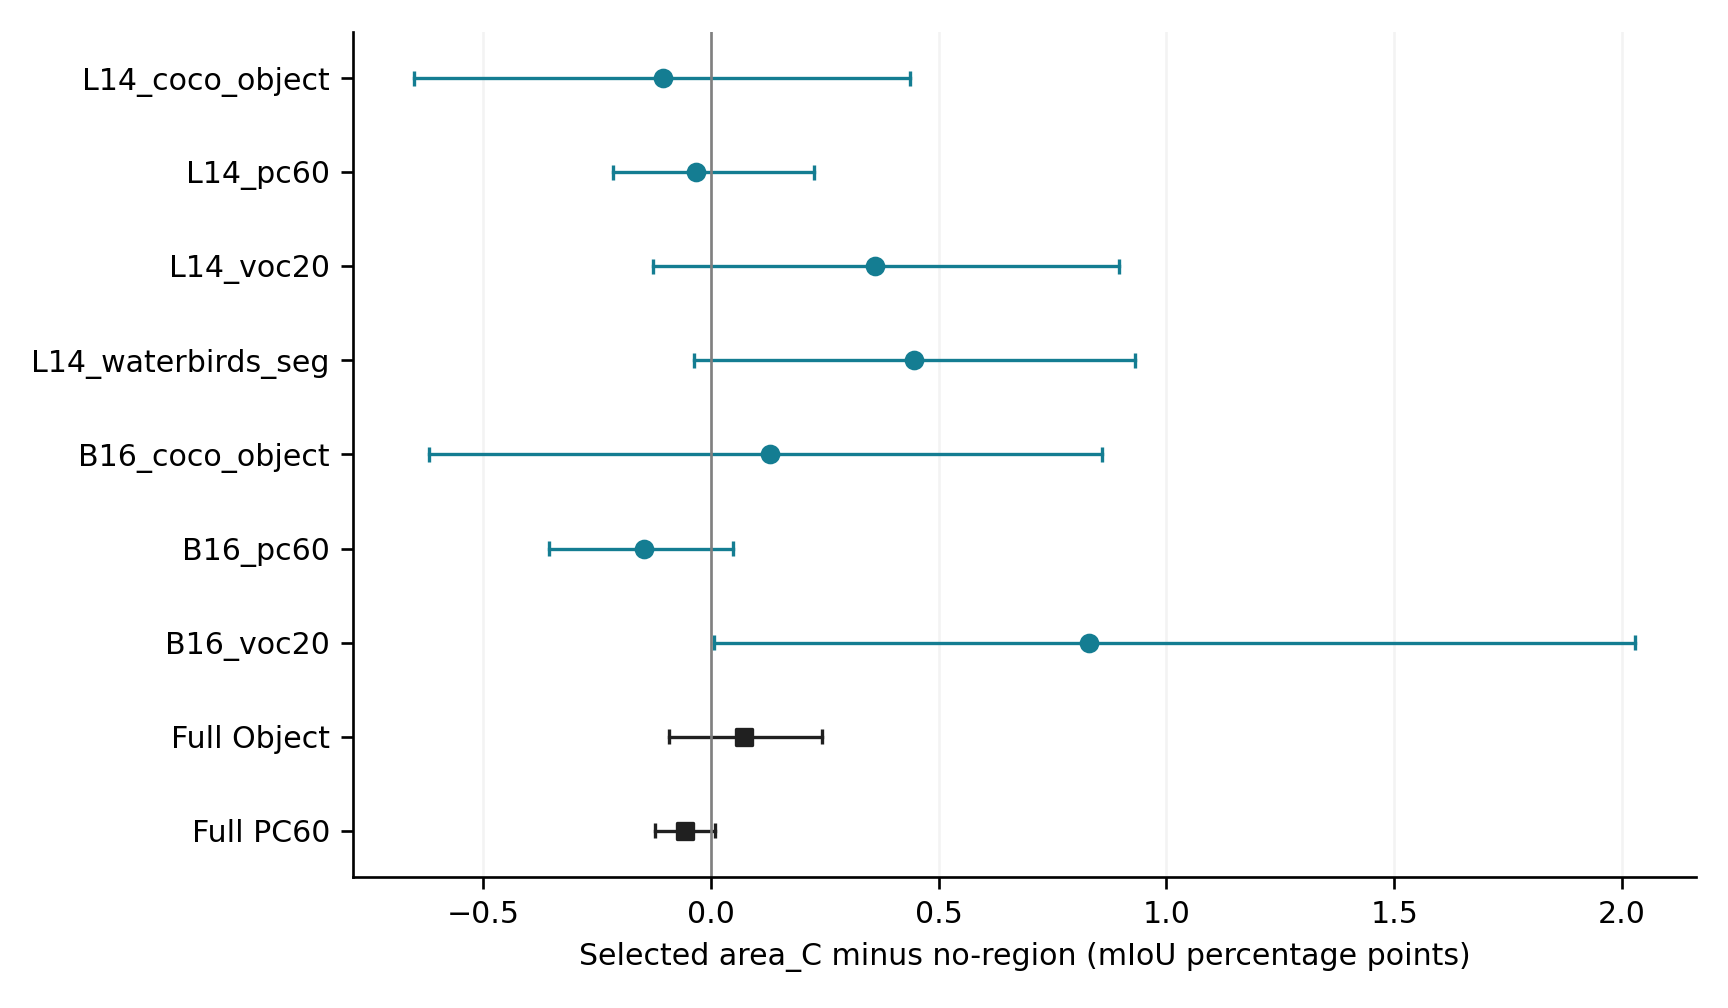
\includegraphics[width=0.97\textwidth]{figures/component_intervals.png}
 \caption{Selected area\_C minus no-region. Teal rows are evaluation-disjoint
 training diagnostics; black squares are the two full-population component
 controls. All intervals are paired, pointwise and unadjusted. Six of seven
 diagnostic intervals and both full-population intervals contain zero.
 The positive B16 VOC20 diagnostic is not a multiplicity-adjusted universal
 mechanism finding.}
 \label{fig:components}
\end{figure*}

Matched-default and selected-system comparisons answer different questions.
The diagnostic default-area addition is nearly null on Object/PC60, whereas
selected operating points change multiple fields. Removing global pixel
entropy hurts Object/PC60 more; CLS removal is more damaging on VOC20 and
Waterbirds. Uniform or spatially shuffled mass can match or exceed C on
several tasks. All 126 cells, including these negative controls, remain in
Tables~\ref{tab:ablations} and~\ref{tab:scores}; no best control replaces the
adopted method after seeing results.

\subsection{Backbone Transfer Is Not Explained by One Bug}
Label-free profiles show larger candidate C and coverage on B16 Object/PC60
(Table~\ref{tab:transfer}). They do not identify a causal explanation for the
accuracy regressions. PC60's first-block regional/global gradient norm ratio
does not increase, and relative parameter-update norms are lower on B16.
Thus a blanket larger-update explanation is unsupported. PC60 has no alias
merge ambiguity, so aliases cannot alone explain all failures. Geometry,
feature distributions and objective interactions remain hypotheses. Gradient
profiles cover only the first fixed eight-source block, with missing ratios
retained; they are not full-population risk predictors.

\subsection{Foreground-Preserving Context Interventions}
R04 constructs 126 of 128 requested COCO cases; two have no eligible supported
instance. All raw/model/native-normalized foreground pixels remain unchanged
across original, sham, hard and edge contexts, without another resize. All
sham predictions are exactly identical. The metric is foreground pixel
accuracy averaged per selected object, not composite-image mIoU.

MLMP scores 71.8265 on original context and 56.8850 after hard replacement;
selected area\_C scores 67.3325 and 57.4963 (Table~\ref{tab:context}). TRACE
minus MLMP is $-4.4941$ points on original views, CI $[-7.9620,-0.9964]$,
and $+0.6113$ on hard replacements with a zero-crossing interval. A smaller
drop from a lower starting accuracy does not establish superior robustness.
Original context is beneficial on average for every method. At the case
level, area\_C has 61 original-beneficial, 51 replacement-beneficial and 14
null hard-replacement outcomes. Neither universal context removal nor a
universal C reliability interpretation follows.

\begin{figure*}[p]
 \centering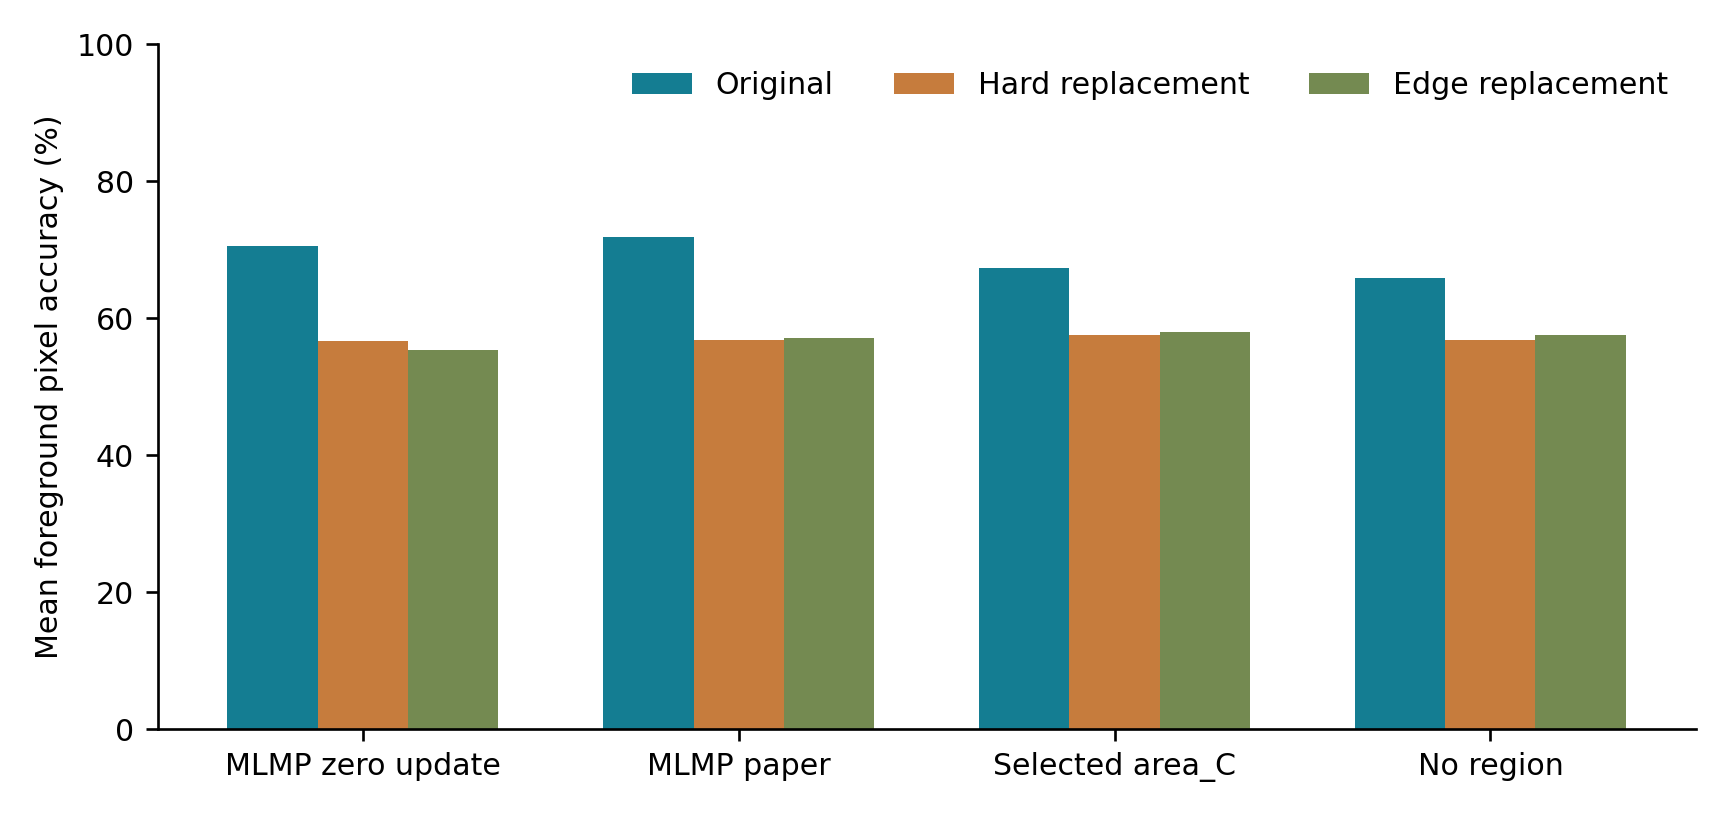
\includegraphics[width=0.97\textwidth]{figures/context_accuracy.png}
 \caption{Mean selected-object foreground accuracy on the controlled context
 set. The zero-based axis preserves the lower original-view starting point of
 area\_C. Exact sham values equal original values and are listed in the table.
 These bars are not full-image segmentation mIoU.}
 \label{fig:context}
\end{figure*}

\subsection{Time-Budget Controls}
The GT-free training pilot measures every integer step from one to twenty in
three arrangements for Object/PC60. It selects the largest integer within
fixed MLMP time in every arrangement: one step on Object and ten on PC60.
Full test results are 30.5268 versus 30.4214 on Object, delta $+0.1054$ with
CI $[-0.0286,0.2248]$, and 27.8738 versus 27.9684 on PC60, delta $-0.0946$
with CI $[-0.3809,0.2047]$ (Table~\ref{tab:time}). Neither establishes an
accuracy improvement. These controls do not replace the main selected
twenty-step Object and five-step PC60 configurations.

Object takes 0.892--0.907 of MLMP time: budget-feasible, but outside strict
$\pm5\%$ near-time equality. PC60 ratios 0.958--0.966 satisfy both criteria.
Formal time and accuracy never reselect steps. Timings include authenticated
input loading/decode, transfer, resets, all probes, updates, readout and host
labels. Model initialization is separate. Diagnostic shared-view timings
and live wrapper/reference CUDA allocations are not intrinsic standalone
speed or memory advantages. Historical time-matching NULL results remain
separate rather than being retroactively relabeled as feasible matches.

\subsection{Historical Risk and Declared Group Outcomes}
The historical R03 isolated-update cohort contains 2042 recorded cases, all
usable, not a new full-population current-method test. All evaluated bootstrap
metrics have zero undefined draws. Grouped OOF
M0 uses confidence/query/class/area; M1 adds C, with optional offline initial
GT-quality controls and a fixed nonlinear M0 sensitivity. All 24 primary
hard-harm metric-increment intervals include zero. A secondary Object
nonlinear quality-adjusted variant worsens Brier and log loss. All 16 AP
increment intervals include zero. These conditional fixed-fit intervals do
not validate calibrated deployment-time update reliability or prove
conditional independence; all results remain in the supplement.

The declared Waterbirds-Seg test yields mean trial worst-group segmentation
mIoU 30.5657/34.1243/37.6249 for NoAdapt/MLMP/area\_C. These are descriptive
group-segmentation points, not classification worst-group accuracy, and no
paired group interval is identified from the original crossed episodes.
The new training diagnostic has group sizes 134/1/1/120, with 3605 undefined
worst-group draws out of 10000; its interval remains unavailable. Balanced
full-test groups do not repair that separate diagnostic uncertainty.

\section{Limitations and Reproducibility}
The principal limitation is scientific attribution: strong selected-system
means do not establish that C supplies the gain. The method adds probe cost,
uses confidence-selected fixed regions, and still performs fixed-step global
updates on low-C images. Simpler mass controls and the two full component
studies constrain the reliability narrative. The evaluation compares the
authorized official MLMP/TENT scope, not every recent OVSS adaptation method,
and does not support a state-of-the-art claim.

Development exposure and unequal calibration remain substantive limits, not
formatting caveats. Corrected PC overlap prevents untouched held-out TRACE
claims; local Waterbirds/COCO-CD populations do not establish independent
public-benchmark generalization. The unresolved Object scalar discrepancy
prevents claiming complete paper-number reproduction. Common-block intervals
condition on fixed runs and many hypotheses; borderline pointwise positives
are not universal mechanistic evidence. We report no causal safety guarantee.

All new science uses one GPU worker and the original shared lock, with
12\,GiB host RAM/1\,GiB swap limits; CPU scoring uses 4\,GiB/1\,GiB, one thread
and hidden CUDA. Complete sealed predictions and successful same-invocation
exits precede each new GT score. A missed corrected-PC loader binding caused
one CPU scoring failure before GT decode; its bytes and journals were retained.
A separately frozen process-local routing repair reused the successful
prediction, verified exact source order and continued only missing stages.
No failed bytes were blindly retried and no successful science was replayed
to find a favorable outcome. All original 96 frozen recovery sources remain
unchanged. The new paper snapshot is independent of protected older papers.

\section{Conclusion}
\method{} provides a completely evaluated training-calibrated operating point
with gains over fixed MLMP on the declared L14 clean and corruption settings
and mixed B16 transfer. The accompanying controls do not establish a
C-specific full-population benefit or an equal-budget accuracy advantage.
Useful context, historical risk-prediction nulls and simpler weighting
controls limit the proposed reliability interpretation. The warranted
conclusion is a bounded system result and an attribution audit, not proof
that context-conditioned support is calibrated update utility.

\FloatBarrier
\clearpage
\bibliographystyle{plainnat}
\bibliography{references}
\clearpage
\onecolumn
\appendix

\section{Complete Main Results}
All values are percentages unless explicitly stated otherwise. Main means
average the upstream rounded per-trial result; exact unrounded means are
also retained. Extension populations and historical exposure are described
in the main protocol. B16 and all fifteen corruptions reuse the corresponding
clean L14 fields without retuning. NoAdapt/TENT and MLMP differ in readout,
so the main comparisons are system-level comparisons.
\begin{table}[htbp]
\centering\scriptsize
\caption{All original fifteen severity-5 corruptions on 1449 sources each. Macro is the arithmetic mean of type means, not pooling condition-images.}
\label{tab:corruptions}
\setlength{\tabcolsep}{4pt}
\begin{tabular}{lrrrrrr}
\toprule
Condition & N & NoAdapt & TENT & MLMP & TRACE & Delta \\
\midrule
L14 S5 brightness & 1449 & 74.9500 & -- & 83.4300 & 85.8700 & +2.4400 \\
L14 S5 contrast & 1449 & 71.5100 & -- & 79.2133 & 81.1300 & +1.9167 \\
L14 S5 defocus\_blur & 1449 & 72.6000 & -- & 80.4167 & 80.6900 & +0.2733 \\
L14 S5 elastic\_transform & 1449 & 62.8700 & -- & 74.0067 & 77.1700 & +3.1633 \\
L14 S5 fog & 1449 & 70.6800 & -- & 79.9067 & 82.8700 & +2.9633 \\
L14 S5 frost & 1449 & 65.3700 & -- & 73.3000 & 76.9500 & +3.6500 \\
L14 S5 gaussian\_noise & 1449 & 62.8800 & -- & 71.1067 & 73.1300 & +2.0233 \\
L14 S5 glass\_blur & 1449 & 71.4500 & -- & 78.7233 & 80.1800 & +1.4567 \\
L14 S5 impulse\_noise & 1449 & 63.1400 & -- & 71.2133 & 72.8300 & +1.6167 \\
L14 S5 jpeg\_compression & 1449 & 72.5900 & -- & 82.1967 & 83.9900 & +1.7933 \\
L14 S5 motion\_blur & 1449 & 73.1000 & -- & 81.2733 & 82.7700 & +1.4967 \\
L14 S5 pixelate & 1449 & 77.2900 & -- & 84.9667 & 86.4900 & +1.5233 \\
L14 S5 shot\_noise & 1449 & 66.2500 & -- & 74.9633 & 77.1900 & +2.2267 \\
L14 S5 snow & 1449 & 71.5000 & -- & 79.4167 & 82.0000 & +2.5833 \\
L14 S5 zoom\_blur & 1449 & 59.0200 & -- & 69.4333 & 71.9400 & +2.5067 \\
15-type macro & 21735 & 69.0133 & -- & 77.5711 & 79.6800 & +2.1089 \\
\bottomrule
\end{tabular}
\end{table}

\FloatBarrier
\begin{table}[htbp]
\centering\scriptsize
\caption{Unrounded exact mIoU means retained separately from official-rounded reporting.}
\label{tab:exact}
\setlength{\tabcolsep}{4pt}
\begin{tabular}{lrrrrrr}
\toprule
Condition & N & NoAdapt & TENT & MLMP & TRACE & Delta \\
\midrule
B16 coco\_object & 5000 & 29.5889 & -- & 30.5281 & 29.7904 & -0.7377 \\
B16 pc60 & 5104 & 28.8990 & -- & 29.6140 & 29.2012 & -0.4129 \\
B16 voc20 & 1449 & 77.5876 & -- & 84.1234 & 84.3786 & +0.2552 \\
L14 coco\_cd & 500 & 62.0626 & -- & 72.3984 & 77.3840 & +4.9856 \\
L14 coco\_object & 5000 & 25.0305 & 26.0533 & 30.4209 & 32.4412 & +2.0202 \\
L14 coco\_stuff & 5000 & 18.3440 & 18.7565 & 21.2489 & 21.9926 & +0.7437 \\
L14 pc59 & 5104 & 28.2300 & 28.7221 & 31.9443 & 32.8746 & +0.9304 \\
L14 pc60 & 5104 & 24.9541 & 25.2802 & 27.9848 & 28.7157 & +0.7310 \\
L14 voc20 & 1449 & 75.9102 & 76.9969 & 83.8048 & 86.1213 & +2.3166 \\
L14 voc21 & 1449 & 45.1307 & 45.6436 & 50.7601 & 51.1429 & +0.3828 \\
L14 waterbirds\_seg & 2568 & 45.3719 & -- & 49.9034 & 54.0250 & +4.1216 \\
L14 S5 brightness & 1449 & 74.9453 & -- & 83.4303 & 85.8671 & +2.4368 \\
L14 S5 contrast & 1449 & 71.5079 & -- & 79.2132 & 81.1329 & +1.9197 \\
L14 S5 defocus\_blur & 1449 & 72.6025 & -- & 80.4171 & 80.6863 & +0.2692 \\
L14 S5 elastic\_transform & 1449 & 62.8682 & -- & 74.0067 & 77.1678 & +3.1611 \\
L14 S5 fog & 1449 & 70.6760 & -- & 79.9069 & 82.8654 & +2.9585 \\
L14 S5 frost & 1449 & 65.3685 & -- & 73.2991 & 76.9514 & +3.6523 \\
L14 S5 gaussian\_noise & 1449 & 62.8773 & -- & 71.1080 & 73.1253 & +2.0173 \\
L14 S5 glass\_blur & 1449 & 71.4451 & -- & 78.7247 & 80.1805 & +1.4558 \\
L14 S5 impulse\_noise & 1449 & 63.1432 & -- & 71.2131 & 72.8270 & +1.6139 \\
L14 S5 jpeg\_compression & 1449 & 72.5902 & -- & 82.1954 & 83.9930 & +1.7976 \\
L14 S5 motion\_blur & 1449 & 73.1001 & -- & 81.2718 & 82.7697 & +1.4979 \\
L14 S5 pixelate & 1449 & 77.2906 & -- & 84.9687 & 86.4945 & +1.5258 \\
L14 S5 shot\_noise & 1449 & 66.2544 & -- & 74.9613 & 77.1916 & +2.2303 \\
L14 S5 snow & 1449 & 71.4955 & -- & 79.4165 & 81.9994 & +2.5829 \\
L14 S5 zoom\_blur & 1449 & 59.0246 & -- & 69.4305 & 71.9390 & +2.5086 \\
\bottomrule
\end{tabular}
\end{table}

\FloatBarrier\clearpage

\section{All Diagnostic Component and Score Controls}
Each family has 256 evaluation-disjoint training sources. L14 and B16 share
source cohorts; orders are not new independent images. All fourteen core
arms and all seven additional score-source controls are shown. The complete
JSON includes every contrast and all bootstrap draws, including interaction
controls; no branch was selected as a new main method.
\begin{table}[htbp]
\centering\scriptsize
\caption{All fourteen core controls on 256 evaluation-disjoint training sources per family; three common-block orders. These are not full-test ablations.}
\label{tab:ablations}
\setlength{\tabcolsep}{4pt}
\begin{tabular}{lrrrrrrr}
\toprule
Control & L14Obj & L14PC & L14VOC & Birds & B16Obj & B16PC & B16VOC \\
\midrule
MLMP & 27.3789 & 27.3666 & 85.1580 & 52.7228 & 26.7469 & 27.4752 & 85.4209 \\
Default area & 27.3559 & 27.3585 & 85.5281 & 53.5278 & 26.7864 & 27.3751 & 85.6407 \\
Selected area & 29.7698 & 27.4814 & 86.4012 & 56.9606 & 26.8762 & 26.5061 & 85.1719 \\
No region & 29.8751 & 27.5148 & 86.0399 & 56.5153 & 26.7458 & 26.6530 & 84.3408 \\
No global & 21.5081 & 24.9032 & 86.5109 & 54.9724 & 24.3581 & 25.5889 & 84.3486 \\
No CLS & 29.1259 & 27.3316 & 83.7738 & 54.6627 & 26.5546 & 26.1514 & 82.8931 \\
No region/CLS & 29.7665 & 27.4428 & 83.0407 & 54.3601 & 26.5030 & 26.3761 & 82.3003 \\
Region-balanced mass & 29.8745 & 27.6537 & 86.0919 & 56.3485 & 26.3574 & 26.6514 & 85.8282 \\
Covered uniform & 30.0884 & 27.4341 & 86.3957 & 56.8866 & 26.6773 & 26.7427 & 85.1568 \\
Image uniform & 30.2061 & 27.5372 & 86.0478 & 56.9545 & 27.0602 & 26.8649 & 84.9910 \\
Spatial shuffle & 30.1805 & 27.6098 & 85.8565 & 57.0430 & 27.0955 & 26.7422 & 84.4041 \\
Semantic top8 & 29.7304 & 27.4814 & 86.2969 & 56.9606 & 26.8121 & 26.5061 & 85.1625 \\
Top4 & 29.7276 & 27.4712 & 86.4135 & 56.8918 & 26.8979 & 26.5976 & 85.0585 \\
Top16 & 29.7993 & 27.3340 & 86.2522 & 56.8538 & 26.9651 & 26.6284 & 85.1321 \\
\bottomrule
\end{tabular}
\end{table}

\begin{table}[htbp]
\centering\scriptsize
\caption{All fixed score-source controls. RegionPLPD is a regional DeYO adaptation; quantile-mapped confidence is not correctness calibration.}
\label{tab:scores}
\setlength{\tabcolsep}{4pt}
\begin{tabular}{lrrrr}
\toprule
Score & L14Obj & L14PC & B16Obj & B16PC \\
\midrule
C & 29.7678 & 27.4760 & 26.7460 & 26.5215 \\
Confidence & 29.4961 & 27.4320 & 26.7509 & 26.7667 \\
RelativeC & 29.7707 & 27.4420 & 26.8064 & 26.5431 \\
ResponseChange & 29.9535 & 27.4556 & 26.8503 & 26.7009 \\
CalibratedConfidence & 29.3696 & 27.5029 & 26.9637 & 26.6680 \\
RegionPLPD & 29.7853 & 27.5383 & 26.7531 & 26.6109 \\
Uniform & 30.0534 & 27.4105 & 26.7596 & 26.7151 \\
\bottomrule
\end{tabular}
\end{table}

\FloatBarrier
\begin{table}[htbp]
\centering\scriptsize
\caption{Prespecified diagnostic contrasts. All other contrasts and all shared bootstrap draws remain in the complete JSON artifact.}
\label{tab:diag-ci}
\setlength{\tabcolsep}{4pt}
\begin{tabular}{lrrrr}
\toprule
Task & Contrast & Delta pp & Pointwise 95\% CI & Undefined \\
\midrule
L14\_coco\_object & default-MLMP & -0.023 & [-0.092, +0.097] & 0 \\
L14\_coco\_object & selected-no region & -0.105 & [-0.650, +0.438] & 0 \\
L14\_coco\_object & selected-image uniform & -0.436 & [-0.932, +0.247] & 0 \\
L14\_coco\_object & selected-shuffle & -0.411 & [-0.853, +0.397] & 0 \\
L14\_pc60 & default-MLMP & -0.008 & [-0.052, +0.076] & 0 \\
L14\_pc60 & selected-no region & -0.033 & [-0.214, +0.226] & 0 \\
L14\_pc60 & selected-image uniform & -0.056 & [-0.324, +0.242] & 0 \\
L14\_pc60 & selected-shuffle & -0.128 & [-0.302, +0.117] & 0 \\
L14\_voc20 & default-MLMP & +0.370 & [+0.096, +0.672] & 0 \\
L14\_voc20 & selected-no region & +0.361 & [-0.128, +0.896] & 0 \\
L14\_voc20 & selected-image uniform & +0.353 & [+0.011, +0.787] & 0 \\
L14\_voc20 & selected-shuffle & +0.545 & [+0.026, +1.244] & 0 \\
L14\_waterbirds\_seg & default-MLMP & +0.805 & [+0.548, +1.074] & 0 \\
L14\_waterbirds\_seg & selected-no region & +0.445 & [-0.037, +0.931] & 0 \\
L14\_waterbirds\_seg & selected-image uniform & +0.006 & [-0.340, +0.351] & 0 \\
L14\_waterbirds\_seg & selected-shuffle & -0.082 & [-0.401, +0.218] & 0 \\
B16\_coco\_object & default-MLMP & +0.039 & [-0.095, +0.174] & 0 \\
B16\_coco\_object & selected-no region & +0.130 & [-0.618, +0.859] & 0 \\
B16\_coco\_object & selected-image uniform & -0.184 & [-0.938, +0.555] & 0 \\
B16\_coco\_object & selected-shuffle & -0.219 & [-0.954, +0.433] & 0 \\
B16\_pc60 & default-MLMP & -0.100 & [-0.192, -0.003] & 0 \\
B16\_pc60 & selected-no region & -0.147 & [-0.356, +0.048] & 0 \\
B16\_pc60 & selected-image uniform & -0.359 & [-0.574, -0.109] & 0 \\
B16\_pc60 & selected-shuffle & -0.236 & [-0.496, +0.037] & 0 \\
B16\_voc20 & default-MLMP & +0.220 & [-0.080, +0.589] & 0 \\
B16\_voc20 & selected-no region & +0.831 & [+0.007, +2.027] & 0 \\
B16\_voc20 & selected-image uniform & +0.181 & [-0.242, +0.628] & 0 \\
B16\_voc20 & selected-shuffle & +0.768 & [-0.095, +1.882] & 0 \\
\bottomrule
\end{tabular}
\end{table}

\FloatBarrier\clearpage

\section{Full Component and Time-Budget Evaluations}
The full component studies keep every selected field fixed except removal
of the regional term. Their common-block episode arrangements are a new
declared post-diagnostic control. In particular, the PC60 mean from this
design is not a replacement for the original shuffled main result.
\begin{table}[htbp]
\centering\scriptsize
\caption{Full-population component control. All 22 selected fields are fixed except explicit regional-loss removal. This is a declared post-diagnostic control, not an untouched preregistered test.}
\label{tab:full-component}
\setlength{\tabcolsep}{4pt}
\begin{tabular}{lrrrrrr}
\toprule
Dataset & N & Full area & No region & Delta pp & Pointwise 95\% CI & Undefined \\
\midrule
Object & 5000 & 32.4412 & 32.3686 & +0.0726 & [-0.092, +0.244] & 0 \\
PC60 & 5104 & 28.8355 & 28.8921 & -0.0566 & [-0.123, +0.010] & 0 \\
\bottomrule
\end{tabular}
\end{table}

\begin{table}[htbp]
\centering\scriptsize
\caption{Full time-budget controls selected without accuracy. Both satisfy the 105\% budget; only PC60 meets the 5\% near-time criterion.}
\label{tab:time}
\setlength{\tabcolsep}{4pt}
\begin{tabular}{lrrrrrr}
\toprule
Dataset & Steps & MLMP & TRACE & Delta pp & Pointwise 95\% CI & Near-time \\
\midrule
Object & 1 & 30.4214 & 30.5268 & +0.1054 & [-0.029, +0.225] & no \\
PC60 & 10 & 27.9684 & 27.8738 & -0.0946 & [-0.381, +0.205] & yes \\
\bottomrule
\end{tabular}
\end{table}

\FloatBarrier
\begin{table}[htbp]
\centering\scriptsize
\caption{All actual training-pilot time ratios relative to fixed paper MLMP. No interpolation or outcome selection.}
\label{tab:time-grid}
\setlength{\tabcolsep}{4pt}
\begin{tabular}{lrrrrrr}
\toprule
Steps & Obj1 & Obj2 & Obj3 & PC1 & PC2 & PC3 \\
\midrule
1 & 0.901 & 0.895 & 0.894 & 0.472 & 0.470 & 0.476 \\
2 & 1.114 & 1.106 & 1.112 & 0.531 & 0.528 & 0.531 \\
3 & 1.326 & 1.311 & 1.309 & 0.582 & 0.583 & 0.591 \\
4 & 1.538 & 1.524 & 1.527 & 0.636 & 0.633 & 0.643 \\
5 & 1.755 & 1.744 & 1.739 & 0.689 & 0.694 & 0.691 \\
6 & 1.964 & 1.953 & 1.943 & 0.748 & 0.742 & 0.753 \\
7 & 2.176 & 2.144 & 2.155 & 0.803 & 0.798 & 0.812 \\
8 & 2.392 & 2.365 & 2.351 & 0.857 & 0.848 & 0.861 \\
9 & 2.579 & 2.572 & 2.567 & 0.911 & 0.899 & 0.923 \\
10 & 2.785 & 2.776 & 2.753 & 0.962 & 0.957 & 0.970 \\
11 & 2.996 & 3.003 & 3.010 & 1.020 & 1.008 & 1.019 \\
12 & 3.196 & 3.232 & 3.207 & 1.077 & 1.068 & 1.077 \\
13 & 3.415 & 3.435 & 3.420 & 1.128 & 1.120 & 1.133 \\
14 & 3.631 & 3.609 & 3.630 & 1.184 & 1.176 & 1.190 \\
15 & 3.851 & 3.805 & 3.818 & 1.233 & 1.228 & 1.245 \\
16 & 4.046 & 4.039 & 4.044 & 1.286 & 1.281 & 1.294 \\
17 & 4.273 & 4.237 & 4.255 & 1.350 & 1.336 & 1.354 \\
18 & 4.488 & 4.454 & 4.460 & 1.397 & 1.391 & 1.409 \\
19 & 4.691 & 4.654 & 4.627 & 1.457 & 1.445 & 1.463 \\
20 & 4.896 & 4.857 & 4.852 & 1.516 & 1.503 & 1.518 \\
\bottomrule
\end{tabular}
\end{table}

\begin{table}[htbp]
\centering\scriptsize
\caption{Selected pilot costs in seconds per source; CUDA peaks in GiB. Initialization is excluded from warm totals and recorded separately. Peaks include live wrapper/reference state and allocator history, not an intrinsic memory advantage.}
\label{tab:cost}
\setlength{\tabcolsep}{4pt}
\begin{tabular}{lrrrrrrrrrr}
\toprule
Task & Arm & Steps & Input & Reset & Probe & Update & Readout & Total & Alloc & Reserve \\
\midrule
L14\_coco\_object & MLMP\_paper & 10 & 0.0027 & 0.0024 & 0.0000 & 0.1251 & 0.0148 & 0.1450 & 3.665 & 3.902 \\
L14\_coco\_object & area\_C & 1 & 0.0029 & 0.0048 & 0.0621 & 0.0367 & 0.0235 & 0.1301 & 3.633 & 3.902 \\
L14\_pc60 & MLMP\_paper & 10 & 0.0023 & 0.0025 & 0.0000 & 0.1250 & 0.0123 & 0.1421 & 2.573 & 3.902 \\
L14\_pc60 & area\_C & 10 & 0.0022 & 0.0013 & 0.0469 & 0.0790 & 0.0074 & 0.1368 & 2.834 & 3.902 \\
\bottomrule
\end{tabular}
\end{table}

\FloatBarrier\clearpage

\section{Complete Context Outcomes}
Requested cases 21 and 102 are unavailable because no supported eligible
instance exists; they are not interpolated or silently replaced. Donors
were outcome-blind. All four contexts preserve the selected foreground,
and exact shams have identical labels. Both helpful and harmful contexts
remain. The MLMP zero-update arm uses its native multi-prompt/layer readout,
not official single-prompt NoAdapt.
\begin{table}[htbp]
\centering\scriptsize
\caption{Selected-instance foreground pixel accuracy (percent), averaged per object and order. Not full-composite mIoU. All sham predictions are exactly identical.}
\label{tab:context}
\setlength{\tabcolsep}{4pt}
\begin{tabular}{lrrrr}
\toprule
Method & Original & Sham & Hard & Edge \\
\midrule
MLMP\_paper & 71.8265 & 71.8265 & 56.8850 & 57.1355 \\
MLMP\_zero\_update & 70.6230 & 70.6230 & 56.7131 & 55.4147 \\
area\_selected & 67.3325 & 67.3325 & 57.4963 & 57.9583 \\
no\_region & 65.9075 & 65.9075 & 56.7841 & 57.4863 \\
\bottomrule
\end{tabular}
\end{table}

\begin{table}[htbp]
\centering\scriptsize
\caption{Observed original-versus-hard replacement outcome strata, not enrollment or donor selection.}
\label{tab:context-benefit}
\setlength{\tabcolsep}{4pt}
\begin{tabular}{lrrr}
\toprule
Method & Original helps & Replacement helps & Null \\
\midrule
MLMP\_paper & 74 & 41 & 11 \\
MLMP\_zero\_update & 79 & 39 & 8 \\
area\_selected & 61 & 51 & 14 \\
no\_region & 62 & 49 & 15 \\
\bottomrule
\end{tabular}
\end{table}

\FloatBarrier
\begin{table}[htbp]
\centering\scriptsize
\caption{All paired context contrasts with identical whole four-source-block bootstrap draws.}
\label{tab:context-ci}
\setlength{\tabcolsep}{4pt}
\begin{tabular}{lrrr}
\toprule
Contrast & Delta pp & Pointwise 95\% CI & Undefined \\
\midrule
MLMP\_paper\_original\_minus\_replacement\_edge & +14.691 & [+9.761, +19.872] & 0 \\
MLMP\_paper\_original\_minus\_replacement\_hard & +14.942 & [+9.005, +21.083] & 0 \\
MLMP\_paper\_original\_minus\_sham & +0.000 & [+0.000, +0.000] & 0 \\
MLMP\_zero\_update\_original\_minus\_replacement\_edge & +15.208 & [+9.918, +20.817] & 0 \\
MLMP\_zero\_update\_original\_minus\_replacement\_hard & +13.910 & [+8.160, +20.205] & 0 \\
MLMP\_zero\_update\_original\_minus\_sham & +0.000 & [+0.000, +0.000] & 0 \\
area\_minus\_MLMP\_original & -4.494 & [-7.962, -0.996] & 0 \\
area\_minus\_MLMP\_replacement\_edge & +0.823 & [-3.228, +5.093] & 0 \\
area\_minus\_MLMP\_replacement\_hard & +0.611 & [-3.521, +4.713] & 0 \\
area\_minus\_MLMP\_sham & -4.494 & [-7.962, -0.996] & 0 \\
area\_minus\_no\_region\_original & +1.425 & [+0.155, +2.804] & 0 \\
area\_minus\_no\_region\_replacement\_edge & +0.472 & [-0.702, +1.407] & 0 \\
area\_minus\_no\_region\_replacement\_hard & +0.712 & [-0.296, +1.800] & 0 \\
area\_minus\_no\_region\_sham & +1.425 & [+0.155, +2.804] & 0 \\
area\_selected\_original\_minus\_replacement\_edge & +9.374 & [+2.943, +16.011] & 0 \\
area\_selected\_original\_minus\_replacement\_hard & +9.836 & [+3.558, +16.205] & 0 \\
area\_selected\_original\_minus\_sham & +0.000 & [+0.000, +0.000] & 0 \\
no\_region\_original\_minus\_replacement\_edge & +8.421 & [+1.809, +15.321] & 0 \\
no\_region\_original\_minus\_replacement\_hard & +9.123 & [+2.570, +15.802] & 0 \\
no\_region\_original\_minus\_sham & +0.000 & [+0.000, +0.000] & 0 \\
\bottomrule
\end{tabular}
\end{table}

\FloatBarrier\clearpage

\section{Group and Backbone Diagnostics}
Local Waterbirds-Seg groups use $g=2y+\mathrm{place}$, with landbird $y=0$
and waterbird $y=1$. The declared test has 642 images in each group. Mask
labels are background/landbird/waterbird. Group mIoU pools source I/U within
each group and omits zero-union classes by the original metric definition;
it need not equal the overall pooled mIoU when averaged across groups.
\begin{table}[htbp]
\centering\scriptsize
\caption{Declared local Waterbirds-Seg test: 642 sources per group. Segmentation mIoU, not classification accuracy. No paired group CI is identified from the crossed original update episodes.}
\label{tab:bird}
\setlength{\tabcolsep}{4pt}
\begin{tabular}{lrrrrr}
\toprule
Method & Group0 & Group1 & Group2 & Group3 & Worst group \\
\midrule
MLMP\_official & 51.5375 & 46.5881 & 40.5237 & 34.1243 & 34.1243 \\
NoAdapt\_official & 47.0106 & 40.4574 & 43.9702 & 30.5657 & 30.5657 \\
area\_C & 51.3298 & 47.9558 & 41.5772 & 37.6249 & 37.6249 \\
\bottomrule
\end{tabular}
\end{table}

\begin{table}[htbp]
\centering\scriptsize
\caption{Label-free descriptive profiles. Candidate statistics cover all diagnostic sources; gradient and update statistics cover only the first fixed eight-source block.}
\label{tab:transfer}
\setlength{\tabcolsep}{4pt}
\begin{tabular}{lrrrrr}
\toprule
Task & C & Coverage & Bonus/grid & Grad ratio & Update L2 \\
\midrule
L14\_coco\_object & 0.3090 & 0.1798 & 0.1175 & 0.1952 & 0.0405 \\
L14\_pc60 & 0.3165 & 0.2674 & 0.1886 & 0.5569 & 0.0308 \\
L14\_voc20 & 0.2904 & 0.4072 & 0.2720 & 0.3710 & 0.0142 \\
L14\_waterbirds\_seg & 0.4076 & 0.7558 & 0.5917 & 0.7471 & 0.0131 \\
B16\_coco\_object & 0.3956 & 0.3948 & 0.2848 & 0.2502 & 0.0343 \\
B16\_pc60 & 0.3901 & 0.4905 & 0.3699 & 0.5466 & 0.0246 \\
B16\_voc20 & 0.3024 & 0.4792 & 0.3236 & 0.2543 & 0.0120 \\
\bottomrule
\end{tabular}
\end{table}

\begin{figure}[htbp]
 \centering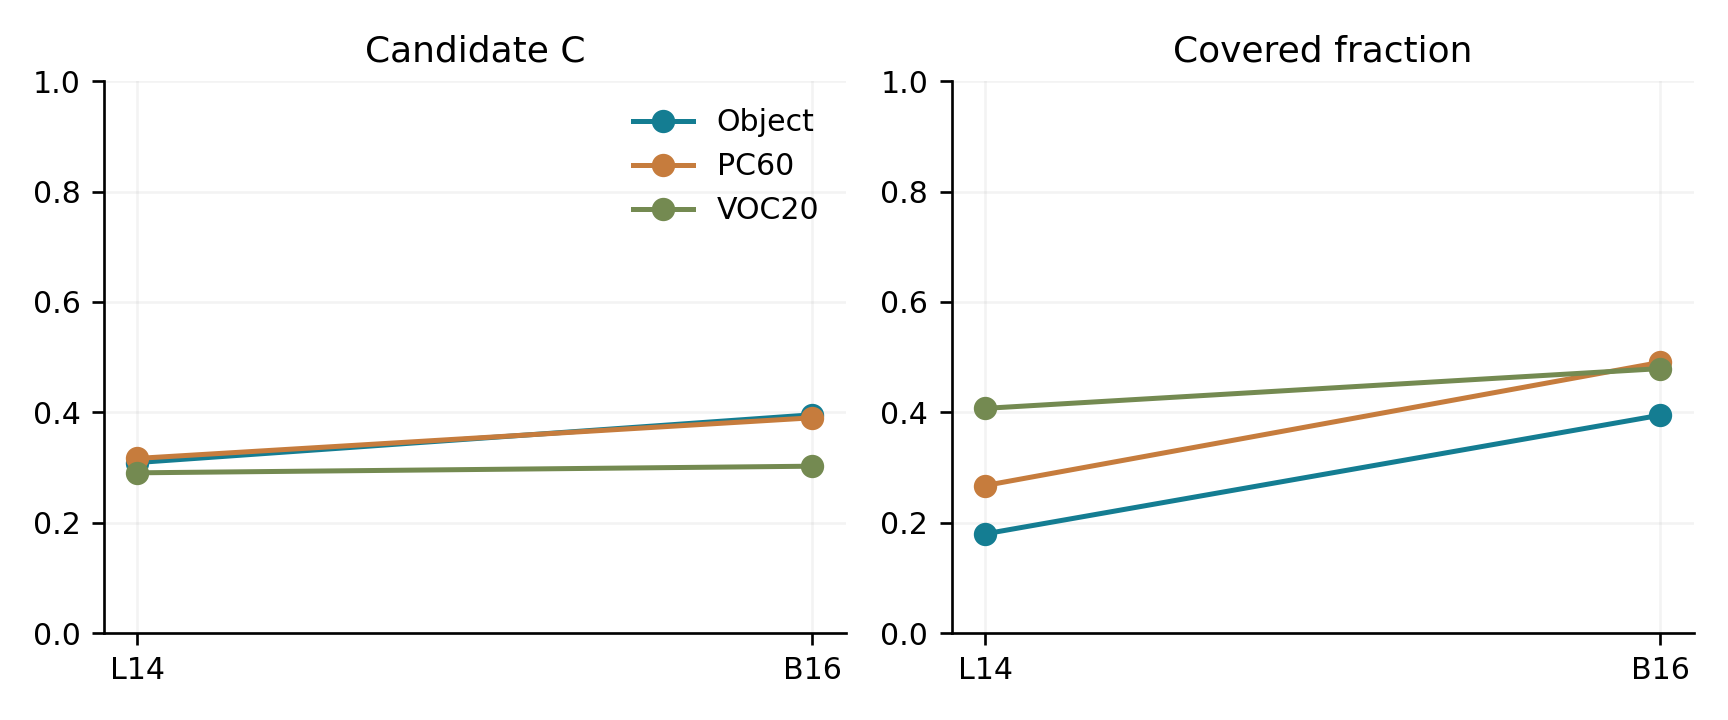
\includegraphics[width=0.88\textwidth]{figures/transfer_profiles.png}
 \caption{Candidate-weighted mean C and image-level coverage on the same
 diagnostic sources. Actual feature-grid areas normalize the L14/B16
 comparison. Lines are descriptive paired profiles, not causal estimates
 or independently calibrated risk.}
 \label{fig:transfer}
\end{figure}
\FloatBarrier\clearpage

\section{All Selected Operating Fields}
Full round-trip precision is in \texttt{complete\_results.json}; displayed
parameter values use compact precision. Batch size is the actual adaptation
batch, not diagnostic-view batch. Diagnostic views use forward batch four.
The final policy selects only from clean L14 training panels and copies
every field to corresponding B16/S5 tasks. Historical B16/S5 development
exposure is not erased by that policy. Zero regional/CLS terms and an identity
probe were diagnostic search controls, not eligible silent replacements
for the adopted method.
\begin{table}[htbp]
\centering\scriptsize
\caption{Selected clean L14 parameters (display precision only); full round-trip values are retained in complete JSON. Every matching B16/S5 field is identical.}
\label{tab:params0}
\setlength{\tabcolsep}{4pt}
\begin{tabular}{lrrrr}
\toprule
Field & coco\_cd & coco\_object & coco\_stuff & pc59 \\
\midrule
C\_power & 1 & 1 & 1 & 1 \\
C\_temperature & 2 & 1 & 2 & 1 \\
adam\_eps & 1e-06 & 1e-08 & 1e-06 & 1e-08 \\
batch\_size & 8 & 1 & 8 & 4 \\
beta1 & 0.9 & 0.9 & 0.9 & 0.9 \\
beta2 & 0.999 & 0.999 & 0.999 & 0.999 \\
candidate\_temperature & 2 & 1 & 2 & 1 \\
channel\_swap & True & True & True & True \\
cls\_temperature & 2 & 1.4142136 & 2 & 1 \\
cls\_weight & 1 & 0.5 & 0.5 & 0.75 \\
connectivity & 8 & 4 & 8 & 4 \\
counterfactual\_contrast & 0 & 0.35 & 0 & 0.35 \\
layer\_fraction & 0.5 & 0.75 & 0.375 & 0.75 \\
lr & 0.01 & 0.0054772256 & 0.0054772256 & 0.01 \\
min\_confidence & 0 & 0 & 0 & 0 \\
min\_region\_area & 8 & 1 & 8 & 1 \\
pixel\_temperature & 0.70710678 & 1 & 1 & 1.4142136 \\
prompt\_count & 7 & 7 & 7 & 3 \\
region\_weight & 4 & 1 & 4 & 1 \\
steps & 5 & 20 & 10 & 5 \\
top\_k & 8 & 8 & 8 & 8 \\
weight\_decay & 0 & 0.0001 & 0 & 0 \\
\bottomrule
\end{tabular}
\end{table}

\begin{table}[htbp]
\centering\scriptsize
\caption{Selected clean L14 parameters (display precision only); full round-trip values are retained in complete JSON. Every matching B16/S5 field is identical.}
\label{tab:params1}
\setlength{\tabcolsep}{4pt}
\begin{tabular}{lrrrr}
\toprule
Field & pc60 & voc20 & voc21 & waterbirds\_seg \\
\midrule
C\_power & 1 & 1 & 1 & 1 \\
C\_temperature & 1 & 1 & 1 & 1 \\
adam\_eps & 1e-08 & 1e-08 & 1e-08 & 1e-08 \\
batch\_size & 4 & 1 & 2 & 2 \\
beta1 & 0.9 & 0.9 & 0.9 & 0.9 \\
beta2 & 0.999 & 0.999 & 0.999 & 0.999 \\
candidate\_temperature & 1 & 1 & 1 & 1 \\
channel\_swap & True & True & True & True \\
cls\_temperature & 2 & 2 & 1 & 1 \\
cls\_weight & 0.75 & 2 & 0.75 & 1 \\
connectivity & 4 & 4 & 4 & 4 \\
counterfactual\_contrast & 0.35 & 0.35 & 0.35 & 0.35 \\
layer\_fraction & 0.75 & 0.75 & 0.75 & 0.75 \\
lr & 0.01 & 0.003 & 0.001 & 0.0017320508 \\
min\_confidence & 0 & 0 & 0 & 0 \\
min\_region\_area & 1 & 1 & 1 & 1 \\
pixel\_temperature & 1 & 1 & 0.70710678 & 1 \\
prompt\_count & 3 & 7 & 7 & 1 \\
region\_weight & 1 & 1 & 2 & 1 \\
steps & 5 & 8 & 20 & 15 \\
top\_k & 8 & 8 & 8 & 8 \\
weight\_decay & 0 & 0 & 0 & 0 \\
\bottomrule
\end{tabular}
\end{table}

\FloatBarrier\clearpage

\section{Current NoAdapt Pairing and Unidentifiable Designs}
The following current-system analysis is distinct from the older image-C
R00 study. It reuses current sealed integer counts only. Old TRACE-minus-MLMP
crossed-order graphs have one connected component in all 26 conditions;
their paired CIs are unidentifiable under the predeclared component rule.
Eligible TRACE-minus-NoAdapt draws share complete dependence blocks across
arms and orders. All fifteen corruption types share the same draws for the
arithmetic macro. This includes prompt/readout changes, not just updates.
\begin{table}[htbp]
\centering\scriptsize
\caption{Current system-level TRACE minus official NoAdapt uncertainty. Unidentifiable designs remain explicit. Not a pure gradient-update effect.}
\label{tab:noadapt-ci}
\setlength{\tabcolsep}{4pt}
\begin{tabular}{lrrr}
\toprule
Condition & Delta pp & Groups & Pointwise 95\% CI \\
\midrule
B16\_coco\_object & +0.201 & 5000 & [-0.580, +0.778] \\
B16\_pc60 & +0.302 & 1 & unidentifiable \\
B16\_voc20 & +6.791 & 1449 & [+5.504, +8.116] \\
L14\_coco\_cd & +15.321 & 1 & unidentifiable \\
L14\_coco\_object & +7.411 & 5000 & [+6.627, +8.013] \\
L14\_coco\_stuff & +3.649 & 1 & unidentifiable \\
L14\_pc59 & +4.645 & 1 & unidentifiable \\
L14\_pc60 & +3.762 & 1 & unidentifiable \\
L14\_voc20 & +10.211 & 1449 & [+8.961, +11.530] \\
L14\_voc20\_C\_brightness & +10.922 & 1449 & [+9.616, +12.246] \\
L14\_voc20\_C\_contrast & +9.625 & 1449 & [+8.156, +11.136] \\
L14\_voc20\_C\_defocus\_blur & +8.084 & 1449 & [+6.537, +9.612] \\
L14\_voc20\_C\_elastic\_transform & +14.300 & 1449 & [+12.574, +16.111] \\
L14\_voc20\_C\_fog & +12.189 & 1449 & [+10.785, +13.626] \\
L14\_voc20\_C\_frost & +11.583 & 1449 & [+9.831, +13.303] \\
L14\_voc20\_C\_gaussian\_noise & +10.248 & 1449 & [+8.513, +11.960] \\
L14\_voc20\_C\_glass\_blur & +8.735 & 1449 & [+7.153, +10.343] \\
L14\_voc20\_C\_impulse\_noise & +9.684 & 1449 & [+8.018, +11.336] \\
L14\_voc20\_C\_jpeg\_compression & +11.403 & 1449 & [+10.127, +12.727] \\
L14\_voc20\_C\_motion\_blur & +9.670 & 1449 & [+8.082, +11.314] \\
L14\_voc20\_C\_pixelate & +9.204 & 1449 & [+7.938, +10.505] \\
L14\_voc20\_C\_shot\_noise & +10.937 & 1449 & [+9.325, +12.500] \\
L14\_voc20\_C\_snow & +10.504 & 1449 & [+9.099, +11.929] \\
L14\_voc20\_C\_zoom\_blur & +12.914 & 1449 & [+11.018, +14.838] \\
L14\_voc21 & +6.012 & 1 & unidentifiable \\
L14\_waterbirds\_seg & +8.653 & 1 & unidentifiable \\
15-type macro & +10.667 & 1449 & [+9.699, +11.636] \\
\bottomrule
\end{tabular}
\end{table}

\FloatBarrier\clearpage

\section{Historical R03: All Prespecified OOF Results}
These are historically selected confidence-TopK isolated unit-weight updates,
not newly generated current area\_C outcomes. Object has 1024 cases from
128 sources/113 original episodes; PC60 has 1018 from 128/105. Five
original-episode grouped folds share training-only preprocessing and fixed
logistic models. Nonlinear M0 uses degree-one-to-three numerical terms;
M1 adds standardized C. Offline GT quality is an adjustment covariate, not
an inference input. Primary harm is negative net correct-pixel change;
the secondary support proxy is not hard prediction harm. AP is
noninterpolated average precision. All 10000 whole-original-episode draws
are retained; each metric has zero undefined draws. Negative Brier/log loss
and positive AP favor M1. These deltas are score units, not percentage points.
\begin{table}[htbp]
\centering\scriptsize
\caption{Historical R03 Brier increments, M1 minus M0 in original score units, not percentage points. Fixed OOF fits; all null/negative results retained.}
\label{tab:r03-brier}
\setlength{\tabcolsep}{4pt}
\begin{tabular}{lrrrrrr}
\toprule
Dataset & Endpoint & M0 & GTquality & Delta & Lower95 & Upper95 \\
\midrule
Object & primary & linear & False & -0.000364 & -0.002227 & +0.001477 \\
Object & primary & linear & True & -0.000040 & -0.001191 & +0.001110 \\
Object & primary & nonlinear & False & -0.000648 & -0.002771 & +0.001479 \\
Object & primary & nonlinear & True & -0.000210 & -0.001452 & +0.001029 \\
Object & secondary\_support & linear & False & +0.000432 & -0.001771 & +0.002758 \\
Object & secondary\_support & linear & True & +0.000462 & -0.000180 & +0.001121 \\
Object & secondary\_support & nonlinear & False & +0.000650 & -0.001393 & +0.002815 \\
Object & secondary\_support & nonlinear & True & +0.000589 & +0.000053 & +0.001153 \\
PC60 & primary & linear & False & +0.000370 & -0.000132 & +0.000934 \\
PC60 & primary & linear & True & +0.000357 & -0.000143 & +0.000906 \\
PC60 & primary & nonlinear & False & +0.000230 & -0.000448 & +0.000950 \\
PC60 & primary & nonlinear & True & +0.000549 & -0.000075 & +0.001168 \\
PC60 & secondary\_support & linear & False & -0.001189 & -0.004337 & +0.001832 \\
PC60 & secondary\_support & linear & True & -0.000116 & -0.000799 & +0.000565 \\
PC60 & secondary\_support & nonlinear & False & -0.001158 & -0.004434 & +0.001988 \\
PC60 & secondary\_support & nonlinear & True & -0.000001 & -0.000544 & +0.000536 \\
\bottomrule
\end{tabular}
\end{table}

\begin{table}[htbp]
\centering\scriptsize
\caption{Historical R03 Log loss increments, M1 minus M0 in original score units, not percentage points. Fixed OOF fits; all null/negative results retained.}
\label{tab:r03-log_loss}
\setlength{\tabcolsep}{4pt}
\begin{tabular}{lrrrrrr}
\toprule
Dataset & Endpoint & M0 & GTquality & Delta & Lower95 & Upper95 \\
\midrule
Object & primary & linear & False & -0.001369 & -0.006348 & +0.003653 \\
Object & primary & linear & True & -0.000262 & -0.003357 & +0.002826 \\
Object & primary & nonlinear & False & +0.001424 & -0.005710 & +0.009849 \\
Object & primary & nonlinear & True & +0.002371 & -0.002294 & +0.008550 \\
Object & secondary\_support & linear & False & -0.000450 & -0.006440 & +0.005730 \\
Object & secondary\_support & linear & True & +0.001276 & -0.000573 & +0.003131 \\
Object & secondary\_support & nonlinear & False & +0.000528 & -0.004950 & +0.006312 \\
Object & secondary\_support & nonlinear & True & +0.001678 & +0.000293 & +0.003150 \\
PC60 & primary & linear & False & +0.000807 & -0.000332 & +0.002038 \\
PC60 & primary & linear & True & +0.000762 & -0.000343 & +0.001963 \\
PC60 & primary & nonlinear & False & +0.000476 & -0.001028 & +0.002067 \\
PC60 & primary & nonlinear & True & +0.001267 & -0.000162 & +0.002671 \\
PC60 & secondary\_support & linear & False & -0.002105 & -0.009333 & +0.004818 \\
PC60 & secondary\_support & linear & True & +0.000563 & -0.001517 & +0.002668 \\
PC60 & secondary\_support & nonlinear & False & -0.001658 & -0.009109 & +0.005554 \\
PC60 & secondary\_support & nonlinear & True & +0.000640 & -0.000960 & +0.002214 \\
\bottomrule
\end{tabular}
\end{table}

\begin{table}[htbp]
\centering\scriptsize
\caption{Historical R03 AP increments, M1 minus M0 in original score units, not percentage points. Fixed OOF fits; all null/negative results retained.}
\label{tab:r03-average_precision}
\setlength{\tabcolsep}{4pt}
\begin{tabular}{lrrrrrr}
\toprule
Dataset & Endpoint & M0 & GTquality & Delta & Lower95 & Upper95 \\
\midrule
Object & primary & linear & False & +0.006183 & -0.002383 & +0.017273 \\
Object & primary & linear & True & +0.001438 & -0.003069 & +0.006227 \\
Object & primary & nonlinear & False & +0.008550 & -0.000562 & +0.020379 \\
Object & primary & nonlinear & True & +0.002421 & -0.004097 & +0.009903 \\
Object & secondary\_support & linear & False & -0.000822 & -0.014950 & +0.013265 \\
Object & secondary\_support & linear & True & -0.002199 & -0.006493 & +0.001275 \\
Object & secondary\_support & nonlinear & False & -0.001378 & -0.014788 & +0.009347 \\
Object & secondary\_support & nonlinear & True & -0.001663 & -0.004056 & +0.000807 \\
PC60 & primary & linear & False & -0.001793 & -0.005207 & +0.001130 \\
PC60 & primary & linear & True & -0.002672 & -0.005924 & +0.000062 \\
PC60 & primary & nonlinear & False & -0.000698 & -0.004344 & +0.002783 \\
PC60 & primary & nonlinear & True & -0.001968 & -0.004649 & +0.000539 \\
PC60 & secondary\_support & linear & False & +0.002025 & -0.006589 & +0.010513 \\
PC60 & secondary\_support & linear & True & -0.002009 & -0.004466 & +0.000435 \\
PC60 & secondary\_support & nonlinear & False & +0.003223 & -0.005131 & +0.011566 \\
PC60 & secondary\_support & nonlinear & True & -0.001660 & -0.004055 & +0.000589 \\
\bottomrule
\end{tabular}
\end{table}

\FloatBarrier\clearpage

\section{Artifact and Execution Index}
The official MLMP source is pinned to commit
\texttt{2a887de018b3f2c3b132f69fe806bab12a2d511f}; DeYO source to
\texttt{3d7d2897d864907571ef75edf31f0028d53f1432}. Local external caches are
not called upstream commits. Source snapshots, input identities, exact
episodes, gates, prediction seals, typed stage admissions and actual process
identities are retained with the results. \texttt{EXPERIMENT\_INDEX.json}
contains complete digests and successful parent bindings. The complete
machine-readable artifact contains all main/ablation/component/context/time/
TENT/group results, shared draws and historical R03 summaries, without raw
RGB, GT, model weights or prediction arrays.

The final recovery controller and final collation exited successfully on
17 November; directory names alone were not accepted as completion.
Successful R04, timing pilot, Object time evaluation and PC60 predictions
were reused by exact identities, not replayed after the loader failure.
The old failed postcontroller, waiting component controller and CPU score
remain failed, with full journals preserved. No resource cap was enlarged,
cache dropped, parallel GPU worker added, or baseline retuned for repair.

Earlier positive/negative/null studies, old V01 infeasible time matches,
failure/cancellation records, geometry distinctions and partial historical
provenance remain valid records of their own scope. R03's original legacy
prediction capture did not include ExecMainCode; that missing historical
field was not invented. Six historical flagged reference-mutation
demonstrations remain not run under platform restrictions; code tests do not
turn them into empirical model gates. No Windows manuscript was supplied or
claimed to have been read. No old paper, raw review, result or main checkout
was overwritten by this independent snapshot.

\end{document}
